\begin{frame}{Validação no LTspice: três configurações}
  \begin{columns}[T,onlytextwidth]
    \begin{column}{0.31\textwidth}
      \centering
      \textbf{Sem carga}

      \vspace{0.14cm}
      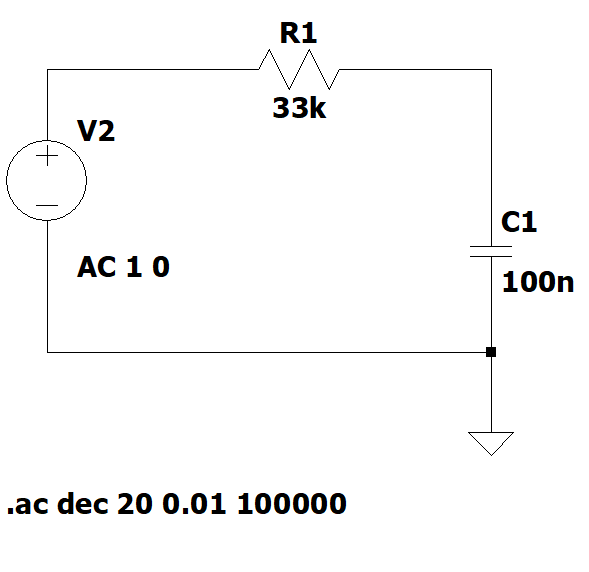
\includegraphics[width=\linewidth,height=0.46\textheight,keepaspectratio]{slides/img/ltspice_circuito_1.png}
    \end{column}
    \begin{column}{0.31\textwidth}
      \centering
      \textbf{Carga direta}

      \vspace{0.14cm}
      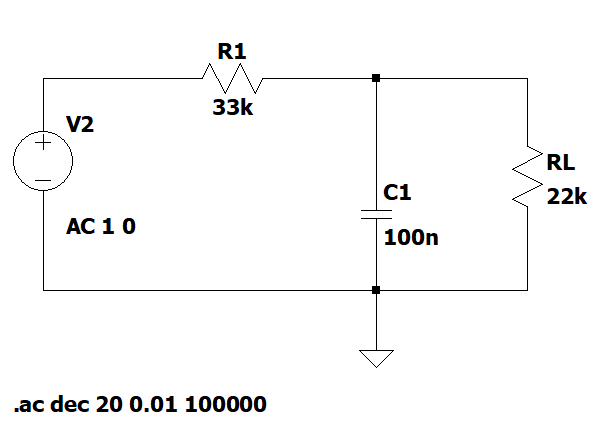
\includegraphics[width=\linewidth,height=0.46\textheight,keepaspectratio]{slides/img/ltspice_circuito_2.png}
    \end{column}
    \begin{column}{0.31\textwidth}
      \centering
      \textbf{Com buffer}

      \vspace{0.14cm}
      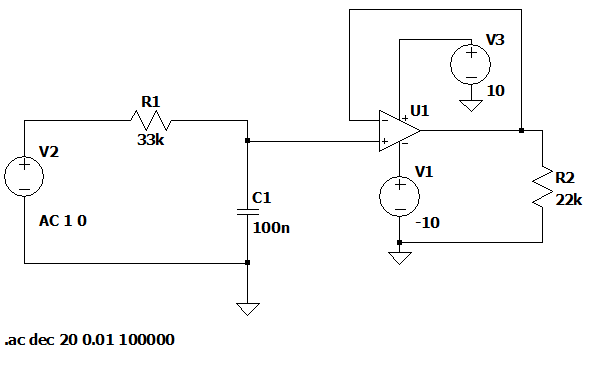
\includegraphics[width=\linewidth,height=0.46\textheight,keepaspectratio]{slides/img/ltspice_circuito_3.png}
    \end{column}
  \end{columns}

  \small
  \begin{block}{Configuração do projeto nominal}
    Entrada AC unitária; varredura de $0{,}01$ a $10^5\,\mathrm{Hz}$, com 20 pontos
    por década. Buffer alimentado em $\pm10\,\mathrm{V}$.
    As capturas utilizam $R=33\,\mathrm{k}\Omega$ e $R_L=22\,\mathrm{k}\Omega$.
  \end{block}
\end{frame}
